\section{DNS}

Existen tres servidores DNS y tres zonas: 
\begin{itemize}	
	\item Mercedes 
	\item Zárate 
	\item	Azul
\end{itemize}

El DNS Root está en la red \textbf{Amapola} de la zona \textbf{Mercedes} con ip 192.168.25.7. Delega la autoridad en los restantes dos 
servidores de nivel dos, por lo que sólo tiene registros NS apuntando hacia los otros servidores DNS de nivel dos. La autoridad de los 
servidores de nivel dos se reparte de la siguiente manera (Ver Figura \ref{dns001}): \\

\begin{itemize}
 \item DNS1, en la red \textbf{Dalia} de la zona \textbf{Azul} con ip 10.111.25.131, para la zona AZUL
 \item DNS2, en la red \textbf{Bergonia} de la zona \textbf{Zárate} con ip 10.111.25.197, para el resto de las zonas
\end{itemize}

\begin{figure}[!htpb]
      \centering
      \begin{center}
      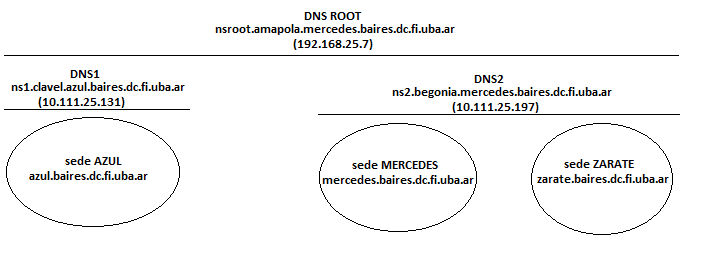
\includegraphics[width=11cm]{Imagenes/dns.png}
      \end{center}
      \caption{Esquema de delegación de dns}
      \label{dns001}
\end{figure}

\indent La parte más compleja de este servidor está en la delegación del mapeo reverso. Se adoptó la práctica común de crear nuevos 
nombres canónicos y hacer a la direcciones IP reales aliases de las primeras, en una relación uno a uno. En conjunto con la creación 
de una zona por cada subnet y la posterior delegación de autoridad sobre esta zona al servidor que se desea que tenga autoridad sobre 
las IPs reales, se logra el cometido. En caso de no estar subneteado, se procede similarmente, delegando cada dirección al nameserver 
correspondiente. Por simplificación se usó el statement \$GENERATE. \\

\indent Es decir, para el mapeo reverso, se creo una zona por cada subnet no alieneada a los objetos de la dirección ip (máscara /24). 
Dentro de esta zona, se delega cada host al servidor DNS de nivel dos correspondiente. El árbol de espacio de nombres de dominios 
(solo teniendo en cuenta los hosts especiales y sus respectivas direciones IPs) se puede apreciar en la Figura \ref{dns002}. \\

\begin{figure}[!htpb]
      \centering
      \begin{center}
      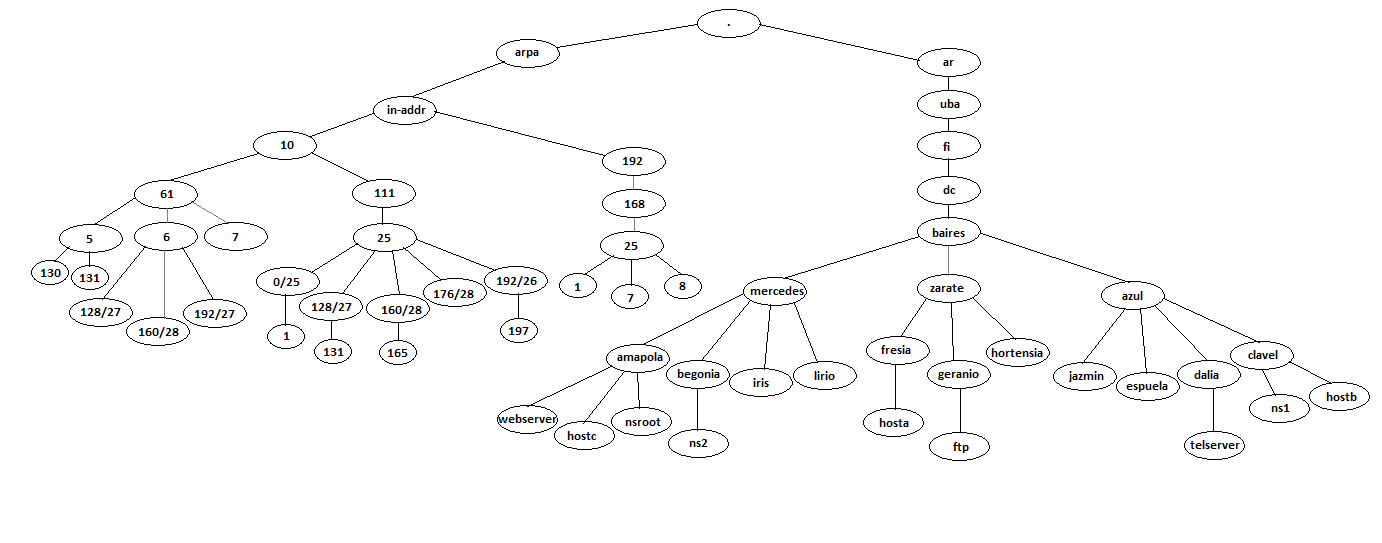
\includegraphics[width=20cm, angle=90]{Imagenes/dns2.png}
      \end{center}
      \caption{Árbol de espacio de nombres de dominio}
      \label{dns002}
\end{figure}


\indent Los host que corren los DNS de nivel tienen como servidor de espacio de nombres al Root, por lo que si se cae este último, los servidores de 
nivel dos serán incapaces de resolver querys incluso para zonas sobre las que tienen autoridad. \\ 

\begin{table}[!htbp]
	\centering
	\begin{tabular}{|c|c|c|c|}   
		\hline
		\multicolumn{4}{|c|}{\textbf{Mercedes}} \\
		\hline
		\hline
		\multicolumn{4}{|c|}{\textbf{Amapola - 192.168.25.0/24 - (.amapola.mercedes.baires.dc.fi.uba.ar)}} \\
		\hline
		Host & Dirección & Nombre & Dominio \\
		\hline
		WebServer & 192.168.25.1 & webserver & www.baires.dc.fi.uba.ar \\
		\hline 
		R1 & 192.168.25.2 & r1 & - \\
		\hline
		R2 & 192.168.25.3 & r2 & - \\
 		\hline
		R3 & 192.168.25.4 & r3 & - \\
		\hline
		R4 & 192.168.25.5 & r4 & - \\
		\hline
		\multirow{2}{*}{DNSRoot} & \multirow{2}{*}{192.168.25.7} & \multirow{2}{*}{nsroot} & ns.baires.dc.fi.uba.ar \\
			& & & nsroot.baires.dc.fi.uba.ar \\
		\hline
		\multirow{2}{*}{HostC} & \multirow{2}{*}{192.168.25.8} & \multirow{2}{*}{hostc} & hostc.baires.dc.fi.uba.ar \\
			& & & c.baires.dc.fi.uba.ar \\
		\hline
		\hline
		\multicolumn{4}{|c|}{\textbf{Begonia - 10.111.25.192/26 - (.begonia.mercedes.baires.dc.fi.uba.ar)}} \\
		\hline
		Host & Dirección & Nombre & Dominio \\
		\hline
		R6 & 10.111.25.193 & r6 & - \\
		\hline
		R18 & 10.111.25.194 & r7 & - \\
		\hline
		DNS2 & 10.111.25.195 & ns2 & ns2.baires.dc.fi.uba.ar \\
		\hline
		\hline
		\multicolumn{4}{|c|}{\textbf{Iris - 10.111.25.176/28 - (.iris.mercedes.baires.dc.fi.uba.ar)}} \\
		\hline
		Host & Dirección & Nombre & Dominio \\
		\hline
		R3 & 10.111.25.177 & r3 & - \\
		\hline
		R4 & 10.111.25.178 & r4 & - \\
		\hline
		\hline
		\multicolumn{4}{|c|}{\textbf{Lirio - 10.61.6.192/27 - (.lirio.mercedes.baires.dc.fi.uba.ar)}} \\
		\hline
		Host & Dirección & Nombre & Dominio \\
		\hline
		R4 & 10.61.6.193 & r4 & - \\
		\hline
		R5 & 10.61.6.194 & r5 & - \\
		\hline
		R6 & 10.61.6.195 & r6 & - \\
		\hline
 	\end{tabular}
	\caption{Esquema de asignaciones en Mercedes}
\end{table}

\begin{table}[!htbp]
	\centering
	\begin{tabular}{|c|c|c|c|}   
		\hline
		\multicolumn{4}{|c|}{\textbf{Azul}} \\
		\hline
		\hline
		\multicolumn{4}{|c|}{\textbf{Clavel - 10.61.5.0/24 - (.clavel.azul.baires.dc.fi.uba.ar)}} \\
		\hline
		Host & Dirección & Nombre & Dominio \\
		\hline
		R16 & 10.61.5.1 & r16 & - \\
		\hline 
		R17 & 10.61.5.2 & r17 & - \\
		\hline
		TelServer & 10.61.5.130 & telserver & telserver.baires.dc.fi.uba.ar \\
 		\hline
		\multirow{2}{*}{Host B} & \multirow{2}{*}{10.61.5.131} & \multirow{2}{*}{hostb} & hostb.baires.dc.fi.uba.ar \\
			& & & b.baires.dc.fi.uba.ar \\
		\hline
		\hline
		\multicolumn{4}{|c|}{\textbf{Dalia - 10.111.25.128/27 - (.dalia.azul.baires.dc.fi.uba.ar)}} \\
		\hline
		Host & Dirección & Nombre & Dominio \\
		\hline
		R17 & 10.111.25.129 & r17 & - \\
		\hline
		R18 & 10.111.25.130 & r18 & - \\
		\hline
		DNS1 & 10.111.25.131 & ns1 & ns1.baires.dc.fi.uba.ar \\
		\hline
		\hline
		\multicolumn{4}{|c|}{\textbf{Espuela - 10.61.6.128/27 - (.espuela.azul.baires.dc.fi.uba.ar)}} \\
		\hline
		Host & Dirección & Nombre & Dominio \\
		\hline
		R14 & 10.61.6.130 & r14 & - \\
		\hline
		R15 & 10.61.6.131 & r15 & - \\
		\hline
		R16 & 10.61.6.132 & r16 & - \\
		\hline
		\hline
		\multicolumn{4}{|c|}{\textbf{Jazmín - 10.61.6.160/28 - (.jazmin.azul.baires.dc.fi.uba.ar)}} \\
		\hline
		Host & Dirección & Nombre & Dominio \\
		\hline
		R18 & 10.61.6.161 & r18 & - \\
		\hline
 	\end{tabular}
	\caption{Esquema de asignaciones en Azul}
\end{table}

\begin{table}[!tbp]
	\centering
	\begin{tabular}{|c|c|c|c|}   
		\hline
		\multicolumn{4}{|c|}{\textbf{Zárate}} \\
		\hline
		\hline
		\multicolumn{4}{|c|}{\textbf{Fresia - 10.111.25.160/28 - (.fresia.zarate.baires.dc.fi.uba.ar)}} \\
		\hline
		Host & Dirección & Nombre & Dominio \\
		\hline
		R10 & 10.111.25.161 & r10 & - \\
		\hline 
		R17 & 10.111.25.162 & r11 & - \\
		\hline
		R12 & 10.111.25.162 & r12 & - \\
		\hline
		R13 & 10.111.25.163 & r13 & - \\
 		\hline
		\multirow{2}{*}{Host C} & \multirow{2}{*}{10.111.25.165} & \multirow{2}{*}{hosta} & hosta.baires.dc.fi.uba.ar \\
			& & & a.baires.dc.fi.uba.ar \\
		\hline
		\hline
		\multicolumn{4}{|c|}{\textbf{Geranio - 10.111.25.0/25 - (.geranio.zarate.dc.fi.uba.ar)}} \\
		\hline
		Host & Dirección & Nombre & Dominio \\
		\hline
		FTP Server & 10.111.25.1 & ftp & ftp.baires.dc.fi.uba.ar \\
		\hline
		R12 & 10.111.25.1 & r12 & - \\
		\hline
		\hline
		\multicolumn{4}{|c|}{\textbf{Hortensia - 10.61.7.128/25 - (.hortensia.zarate.baires.dc.fi.uba.ar)}} \\
		\hline
		Host & Dirección & Nombre & Dominio \\
		\hline
		R7 & 10.61.7.129 & r7 & - \\
		\hline
		R9 & 10.61.7.130 & r8 & - \\
		\hline
		R10 & 10.61.7.131 & r10 & - \\
		\hline
		R11 & 10.61.7.132 & r12 & - \\
		\hline
 	\end{tabular}
	\caption{Esquema de asignaciones en Zárate}
\end{table}
